\documentclass[border=25pt, tikz]{standalone}
\usetikzlibrary{shapes.geometric, arrows.meta, positioning, calc, backgrounds}

\begin{document}
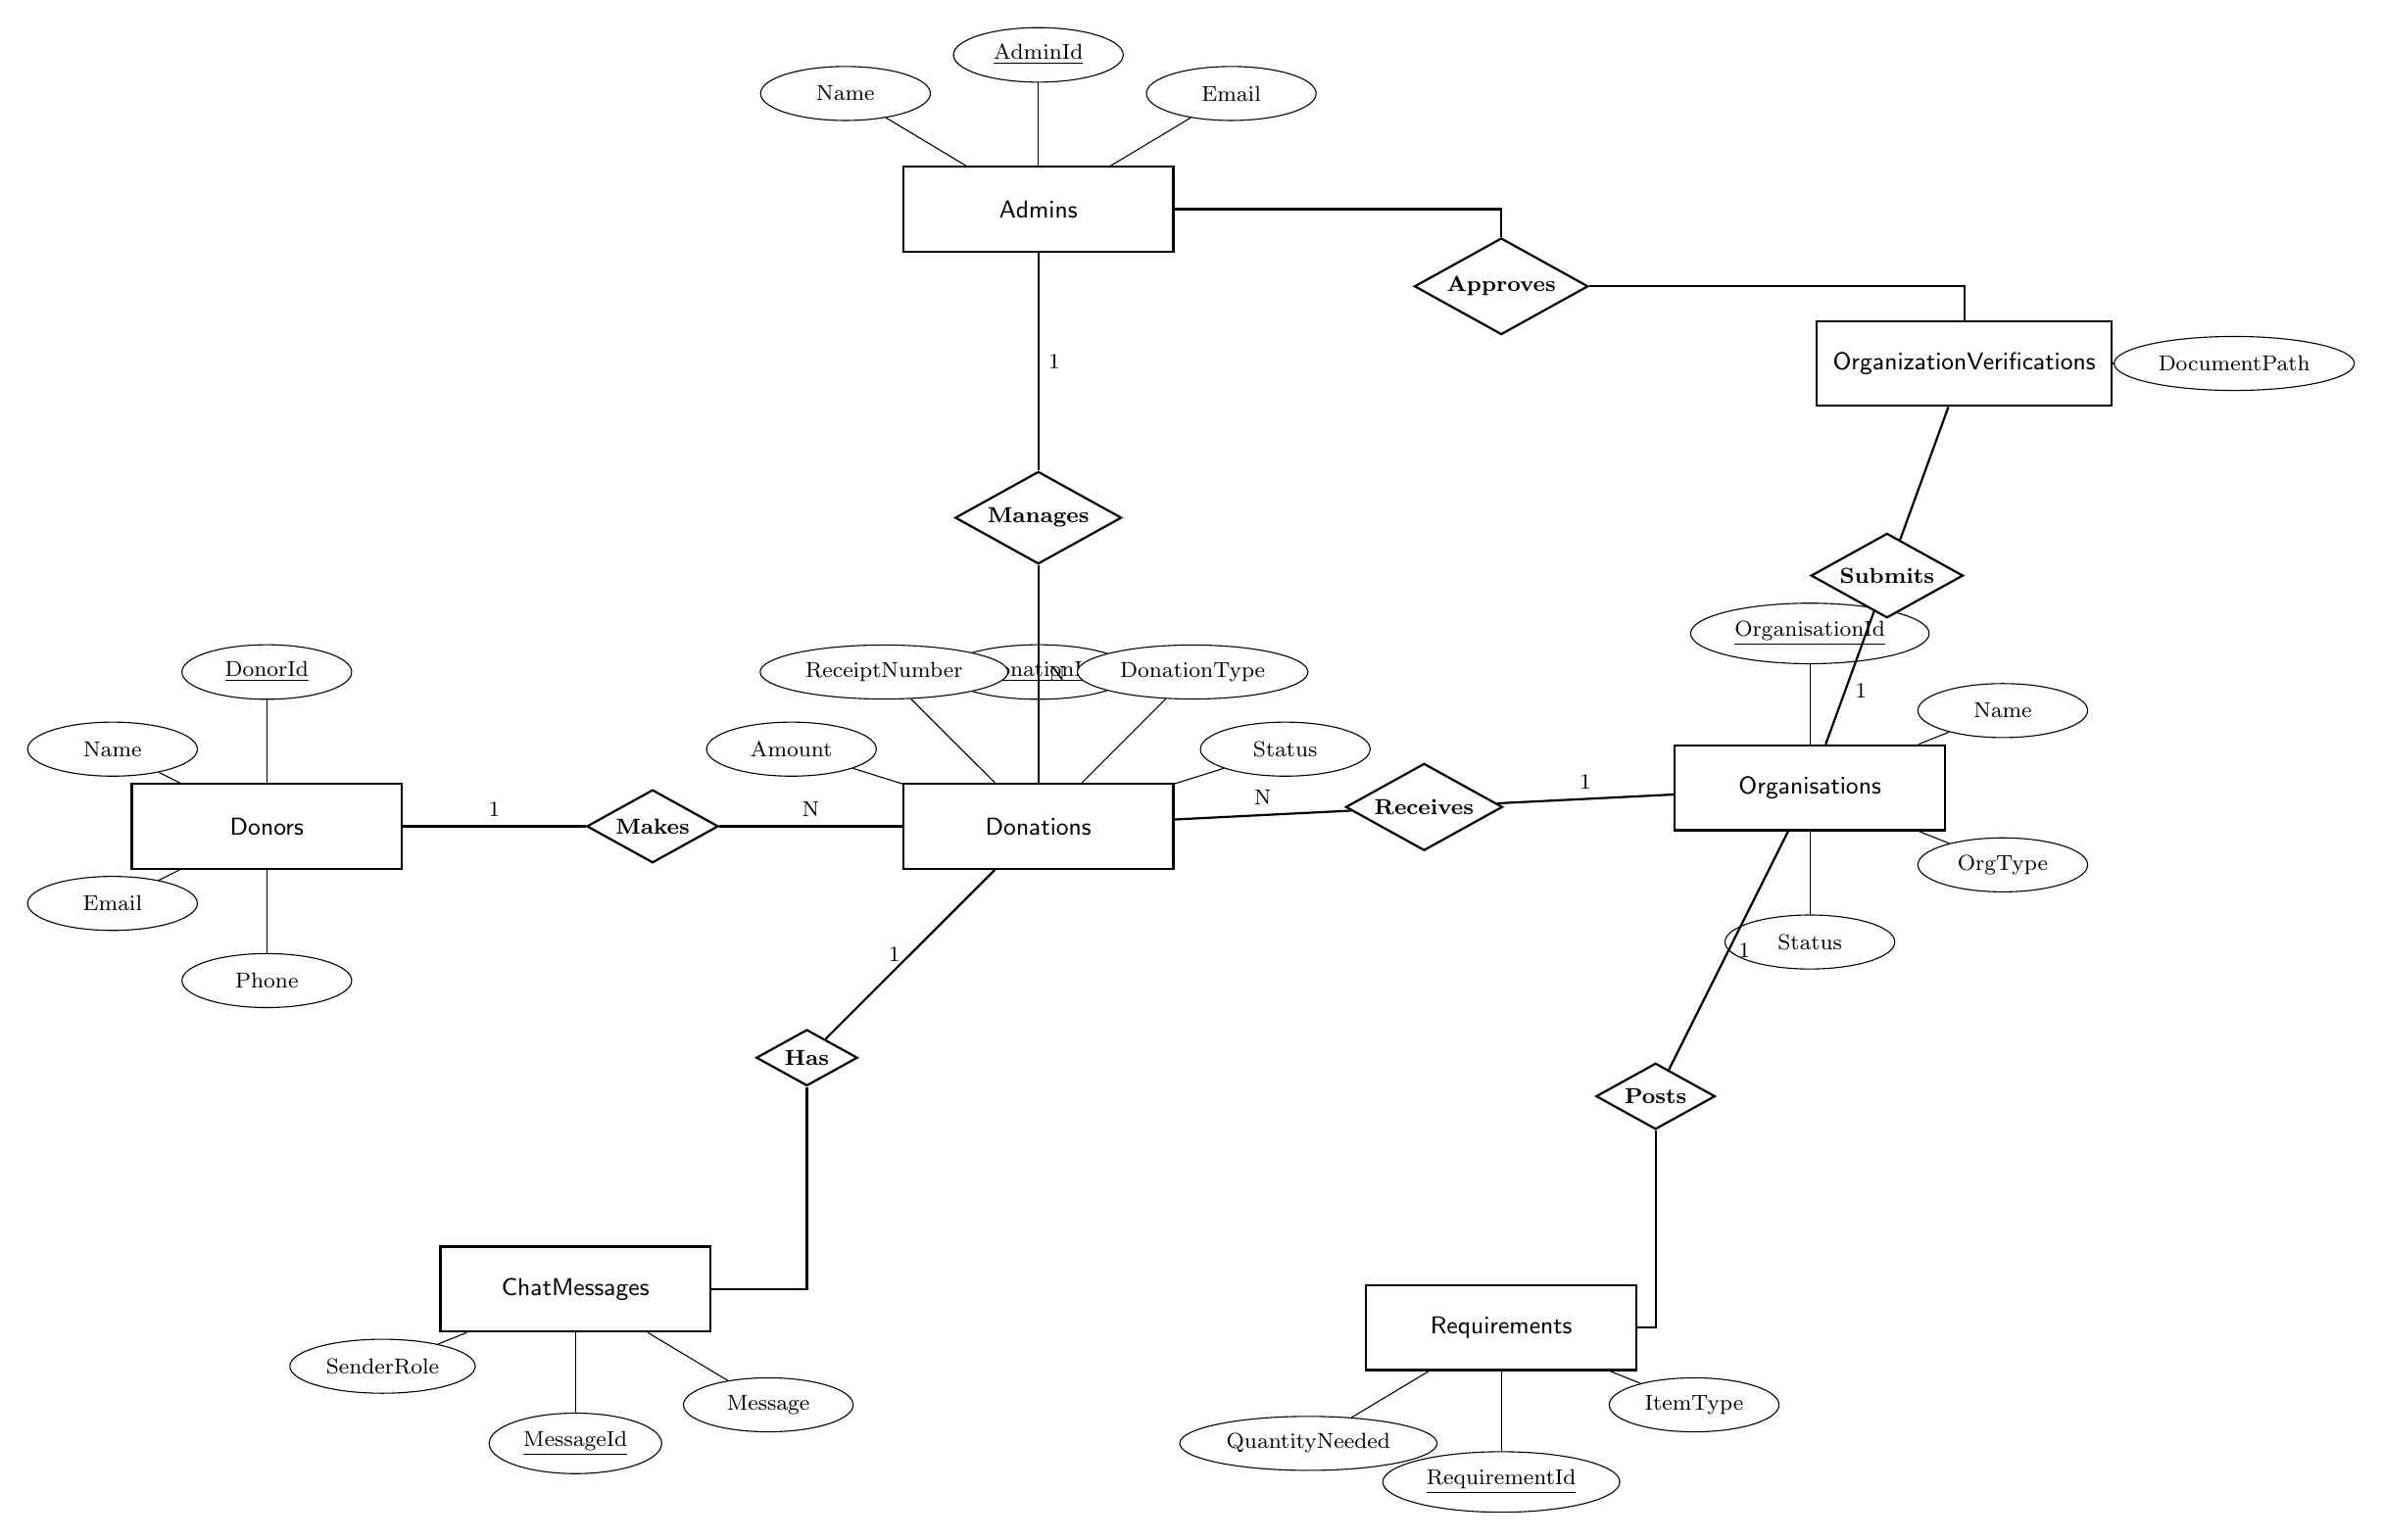
\begin{tikzpicture}[
    font=\sffamily\small,
    entity/.style={
        rectangle, draw=black, thick, 
        fill=white, 
        minimum width=3.5cm, minimum height=1.1cm, align=center,
        inner sep=6pt
    },
    attribute/.style={
        ellipse, draw=black, thin, 
        fill=white, 
        minimum width=2.2cm, minimum height=0.7cm, align=center, font=\footnotesize
    },
    relationship/.style={
        diamond, draw=black, thick, 
        fill=white, 
        aspect=1.8, align=center, inner sep=2pt, font=\footnotesize\bfseries
    },
    line/.style={draw=black, thick}
]

% ---------------------------------------------------------------------
% 1. CENTER: DONATIONS
% ---------------------------------------------------------------------
\node[entity] (Donations) at (0, 0) {Donations};

% Donation attributes - Fanned out to not block lines
\node[attribute] (Don1) at (0, 2) {\underline{DonationId}};
\node[attribute] (Don2) at (-2, 2) {ReceiptNumber};
\node[attribute] (Don3) at (2, 2) {DonationType};
\node[attribute] (Don4) at (-3.2, 1) {Amount};
\node[attribute] (Don5) at (3.2, 1) {Status};

\draw (Donations) -- (Don1); \draw (Donations) -- (Don2); \draw (Donations) -- (Don3); 
\draw (Donations) -- (Don4); \draw (Donations) -- (Don5);

% ---------------------------------------------------------------------
% 2. LEFT: DONORS
% ---------------------------------------------------------------------
\node[entity] (Donors) at (-10, 0) {Donors};

% Donor attributes
\node[attribute] (Dor1) at (-10, 2) {\underline{DonorId}};
\node[attribute] (Dor2) at (-12, 1) {Name};
\node[attribute] (Dor3) at (-12, -1) {Email};
\node[attribute] (Dor4) at (-10, -2) {Phone};

\draw (Donors) -- (Dor1); \draw (Donors) -- (Dor2); \draw (Donors) -- (Dor3); \draw (Donors) -- (Dor4);

% ---------------------------------------------------------------------
% 3. RIGHT: ORGANISATIONS
% ---------------------------------------------------------------------
\node[entity] (Organisations) at (10, 0.5) {Organisations};

% Organisation attributes
\node[attribute] (Org1) at (10, 2.5) {\underline{OrganisationId}};
\node[attribute] (Org2) at (12.5, 1.5) {Name};
\node[attribute] (Org3) at (12.5, -0.5) {OrgType};
\node[attribute] (Org4) at (10, -1.5) {Status};

\draw (Organisations) -- (Org1); \draw (Organisations) -- (Org2); \draw (Organisations) -- (Org3); \draw (Organisations) -- (Org4);

% ---------------------------------------------------------------------
% 4. TOP: ADMINS
% ---------------------------------------------------------------------
\node[entity] (Admins) at (0, 8) {Admins};

% Admin attributes
\node[attribute] (Adm1) at (0, 10) {\underline{AdminId}};
\node[attribute] (Adm2) at (-2.5, 9.5) {Name};
\node[attribute] (Adm3) at (2.5, 9.5) {Email};

\draw (Admins) -- (Adm1); \draw (Admins) -- (Adm2); \draw (Admins) -- (Adm3);

% ---------------------------------------------------------------------
% 5. BOTTOM LEFT: CHATMESSAGES
% ---------------------------------------------------------------------
\node[entity] (ChatMessages) at (-6, -6) {ChatMessages};

% Chat attributes
\node[attribute] (Chat1) at (-6, -8) {\underline{MessageId}};
\node[attribute] (Chat2) at (-8.5, -7) {SenderRole};
\node[attribute] (Chat3) at (-3.5, -7.5) {Message};

\draw (ChatMessages) -- (Chat1); \draw (ChatMessages) -- (Chat2); \draw (ChatMessages) -- (Chat3);

% ---------------------------------------------------------------------
% 6. BOTTOM RIGHT: REQUIREMENTS
% ---------------------------------------------------------------------
\node[entity] (Requirements) at (6, -6.5) {Requirements};

% Requirement attributes
\node[attribute] (Req1) at (6, -8.5) {\underline{RequirementId}};
\node[attribute] (Req2) at (8.5, -7.5) {ItemType};
\node[attribute] (Req3) at (3.5, -8) {QuantityNeeded};

\draw (Requirements) -- (Req1); \draw (Requirements) -- (Req2); \draw (Requirements) -- (Req3);

% ---------------------------------------------------------------------
% 7. MID-RIGHT: VERIFICATIONS
% ---------------------------------------------------------------------
\node[entity] (Verifications) at (12, 6) {OrganizationVerifications};
\node[attribute] (Ver1) at (15.5, 6) {DocumentPath};
\draw (Verifications) -- (Ver1);

% ---------------------------------------------------------------------
% RELATIONSHIPS (Increased Path Spacing)
% ---------------------------------------------------------------------

% Donor -> Makes -> Donation
\node[relationship] (Rel1) at (-5, 0) {Makes};
\draw[line] (Donors) -- node[above, font=\footnotesize] {1} (Rel1) -- node[above, font=\footnotesize] {N} (Donations);

% Org -> Receives -> Donation
\node[relationship] (Rel2) at (5, 0.25) {Receives};
\draw[line] (Organisations) -- node[above, font=\footnotesize] {1} (Rel2) -- node[above, font=\footnotesize] {N} (Donations);

% Donation -> Has -> Chat
\node[relationship] (Rel3) at (-3, -3) {Has};
\draw[line] (Donations) -- node[left, font=\footnotesize] {1} (Rel3);
\draw[line] (Rel3) |- (ChatMessages);

% Org -> Posts -> Requirements
\node[relationship] (Rel4) at (8, -3.5) {Posts};
\draw[line] (Organisations) -- node[right, font=\footnotesize] {1} (Rel4);
\draw[line] (Rel4) |- (Requirements);

% Org -> Submits -> Verifications
\node[relationship] (Rel5) at (11, 3.25) {Submits};
\draw[line] (Organisations) -- node[right, pos=0.4, font=\footnotesize] {1} (Rel5);
\draw[line] (Rel5) -- (Verifications);

% Admin -> Manages -> Donations
\node[relationship] (Rel6) at (0, 4) {Manages};
\draw[line] (Admins) -- node[right, font=\footnotesize] {1} (Rel6) -- node[right, font=\footnotesize] {N} (Donations);

% Admin -> Approves -> Verifications
\node[relationship] (Rel7) at (6, 7) {Approves};
\draw[line] (Admins) -| (Rel7);
\draw[line] (Rel7) -- (12, 7) -- (Verifications);

\end{tikzpicture}
\end{document}
